% Copyright 2007, 2008, 2009 Elsevier Ltd
%% 
%% This file is part of the 'Elsarticle Bundle'.
%% ---------------------------------------------
%% 
%% It may be distributed under the conditions of the LaTeX Project Public
%% License, either version 1.2 of this license or (at your option) any
%% later version.  The latest version of this license is in
%%    http://www.latex-project.org/lppl.txt
%% and version 1.2 or later is part of all distributions of LaTeX
%% version 1999/12/01 or later.
%% 
%% The list of all files belonging to the 'Elsarticle Bundle' is
%% given in the file `manifest.txt'.
%% 
%% Template article for Elsevier's document class `elsarticle'
%% with harvard style bibliographic references
%% SP 2008/03/01

\documentclass[review, 12pt]{elsarticle}
%\documentclass{elsart1p}

%% Use the option review to obtain double line spacing
%% \documentclass[authoryear,preprint,review,12pt]{elsarticle}

%% Use the options 1p,twocolumn; 3p; 3p,twocolumn; 5p; or 5p,twocolumn
%% for a journal layout:
%% \documentclass[final,1p,times,authoryear]{elsarticle}
%% \documentclass[final,1p,times,twocolumn,authoryear]{elsarticle}
%% \documentclass[final,3p,times,authoryear]{elsarticle}
%% \documentclass[final,3p,times,twocolumn,authoryear]{elsarticle}
%% \documentclass[final,5p,times,authoryear]{elsarticle}

%% For including figures, graphicx.sty has been loaded in
%% elsarticle.cls. If you prefer to use the old commands
%% please give \usepackage{epsfig}

%% The amssymb package provides various useful mathematical symbols
%% The amsthm package provides extended theorem environments
%% \usepackage{amsthm}

%% The lineno packages adds line numbers. Start line numbering with
%% \begin{linenumbers}, end it with \end{linenumbers}. Or switch it on
%% for the whole article with \linenumbers.
%% \usepackage{lineno}

%*******************************************************
%% Add packages
%*******************************************************
\usepackage{extsizes}
%\usepackage[super,sort&compress,comma]{natbib} 
\usepackage[left=1.5cm, right=1.5cm, top=1.785cm, bottom=2.0cm]{geometry}
\usepackage{balance}
\usepackage{mathptmx}
\usepackage{sectsty}
\usepackage{graphicx} 
\usepackage{lastpage}
\usepackage[format=plain,justification=justified,singlelinecheck=false,font={stretch=1.125,small,sf},labelfont=bf,labelsep=space]{caption}
\usepackage{float}
\usepackage{fancyhdr}
\usepackage{amsmath}
\usepackage{booktabs} %
\numberwithin{equation}{section}

\usepackage{fnpos}
\usepackage[english]{babel}
\addto{\captionsenglish}{%
  \renewcommand{\refname}{Notes and references}
}
\usepackage{array}
\usepackage{droidsans}
\usepackage{charter}
\usepackage[T1]{fontenc}
\usepackage[usenames,dvipsnames]{xcolor}
\usepackage{setspace}
\usepackage[compact]{titlesec}
\usepackage{hyperref}
\usepackage{amsmath,amsthm, amssymb} % New
\usepackage{gensymb}
\usepackage{enumerate} % New added
\usepackage{subfig} % New added
\usepackage{color} % New added
\usepackage{xspace} % New added
\usepackage{array} % New added
\usepackage{braket} % New added
\usepackage{ulem}
\usepackage{relsize}
\usepackage{tabularx}
%\usepackage[nodisplayskipstretch]{setspace}
\usepackage{bm} 
%\usepackage{epstopdf} %converting to PDF
%\usepackage{array}
%\newcolumntype{P}[1]{>{\centering\arraybackslash}p{#1}}
%%%Please don't disable any packages in the preamble, as this may cause the template to display incorrectly.%%%
%\usepackage{epstopdf}%This line makes .eps figures into .pdf - please comment out if not required.
\definecolor{cream}{RGB}{222,217,201}
%%%%%%%%% Preamble of the bibliography, can be commented or deleted 


%*******************************************************
%Commands to be used regularly % New added
%*******************************************************
\newcommand{\myfloatalign}{\centering} % how all the floats will be aligned
\renewcommand{\bold}[1]{\boldsymbol{#1}} % for boldsymbols
\newcommand{\xt}{(\bold{x},t)}
\newcommand{\lxt}{(x,t)} % xt for x-dimension 
\renewcommand{\sp}[1]{\left({#1}\right)} % for small parentheses 
\let\vaccent=\v % rename builtin command \v{ to \vaccent{
\renewcommand{\v}[1]{\ensuremath{\mathbf{#1}}} % for vectors
\newcommand{\m}[1]{\ensuremath{\mathrm{#1}}} % for dyadic product of vectors 
\newcommand{\gv}[1]{\ensuremath{\mbox{\boldmath$ #1 $}}}
% for vectors of Greek letters
\newcommand{\uv}[1]{\ensuremath{\mathbf{\hat{#1}}}} % for unit vector
\newcommand{\abs}[1]{\left| #1 \right|} % for absolute value
\newcommand{\avg}[1]{\left< #1 \right>} % for average
\let\underdot=\d % rename builtin command \d{ to \underdot{
\renewcommand{\d}[2]{\frac{d #1}{d #2}} % for derivatives
\newcommand{\dd}[2]{\frac{d^2 #1}{d #2^2}} % for double derivatives
\newcommand{\pd}[2]{\frac{\partial #1}{\partial #2}} % for partial derivatives
\newcommand{\pdd}[2]{\frac{\partial^2 #1}{\partial #2^2}} % for double partial derivatives d2y/dx2
\newcommand{\pddm}[3]{\frac{\partial^2 #1}{{\partial #2} {\partial #3}}} % for doubl partial derivatives d2y/dxdy
\newcommand{\pdc}[3]{\left( \frac{\partial #1}{\partial #2}\right)_{#3}} % for thermodynamic partial derivatives
\newcommand{\matrixel}[3]{\left< #1 \vphantom{#2#3} \right|
     #2 \left| #3 \vphantom{#1#2} \right>} % for Dirac matrix elements
\newcommand{\grad}[1]{\gv{\nabla} #1} % for gradient
\let\divsymb=\div % rename builtin command \div to \divsymb
\renewcommand{\div}[1]{\gv{\nabla} \cdot #1} % for divergence
\newcommand{\curl}[1]{\gv{\nabla} \times #1} % for curl
\providecommand{\norm}[1]{\lVert#1\rVert}
\newcommand{\mode}{\!\left(\substack{\gv{k} \\ \nu}\right)}
\newcommand{\modet}{\!\left(\substack{\gv{\kappa} \\ \nu};t\right)}
\newcommand{\modeomega}{\!\left(\substack{\gv{\kappa} \\ \nu};\omega\right)}
\newcommand{\amit}[1]{{\color{red} (Amit's Comment: #1)}}
\newcommand{\abhikeern}[1]{{\color{red} #1}}
\newcommand{\change}[1]{{\color{red} #1}}
\newcommand {\eqn}[1] {Eq.~(\ref{#1})}
\newcommand {\eqns}[1] {Eqs.~(\ref{#1})}
\newcommand {\eqnx}[1] {(\ref{#1})}
\newcommand {\Eqn}[1] {Equation~(\ref{#1})}
\newcommand {\sect}[1] {Section~\ref{#1}}
\newcommand {\app}[1] {Appendix~\ref{#1}}
\newcommand {\fig}[1] {Fig.~\ref{#1}}
\newcommand {\Fig}[1] {Figure~\ref{#1}}
\newcommand {\figs}[1] {Figs.~\ref{#1}}
\newcommand {\figx}[1] {\ref{#1}}
\newcommand {\refcite}[1] {Ref.~[\onlinecite{#1}]}
\newcommand {\refcites}[1] {Refs.~[\onlinecite{#1}]}
\newcommand {\refcitex}[1] {[\onlinecite{#1}]}
\newcommand{\sumdd}[3]{\ensuremath{\sum_{\substack{#1 \\ #2}}^{#3}}}
\newcommand{\tL}{\theta_{\rm L}}
\newcommand{\tR}{\theta_{\rm R}}
\newcommand{\nbins}{N_{\rm bins}}
\newcommand{\deltmd}{\Delta t_{\rm MD}}


%%%%%%%%%%%%%%%%%%%%%%%%%%%%%%%%%%%%%%%%%%%%%%%%%%%%%%%%%%%%%%%%



\makeatletter
\def\@author#1{\g@addto@macro\elsauthors{\normalsize%
    \def\baselinestretch{1}%
    \upshape\authorsep#1\unskip\textsuperscript{%
      \ifx\@fnmark\@empty\else\unskip\sep\@fnmark\let\sep=,\fi
      \ifx\@corref\@empty\else\unskip\sep\@corref\let\sep=,\fi
      }%
    \def\authorsep{\unskip,\space}%
    \global\let\@fnmark\@empty
    \global\let\@corref\@empty  %% Added
    \global\let\sep\@empty}%
    \@eadauthor={#1}
}
\makeatother


\doublespacing
\journal{*******}

\begin{document}

\begin{frontmatter}

\title{Benchmarking Neural Equivariant Potentials for Mechanical Response of Amorphous Boron Nitride}

\author{Ashwani Kushwaha}
\ead{193100026@iitb.ac.in}
\author{Amit Singh\corref{cor1}}
\ead{amit.k.singh@iitb.ac.in}
\cortext[cor1]{Corresponding author}
\address{Department of Mechanical Engineering, IIT Bombay, Mumbai 400076, India}


\date{\today}

\begin{abstract}
Amorphous boron nitride (a-BN) is an important insulating material for advanced electronic applications, yet its mechanical behavior remains challenging to characterize due to structural disorder and complex bonding environments. In this work, we assess the capability of neural equivariant interatomic potentials (NEPs) to model the mechanical response of a-BN using molecular dynamics simulations within the LAMMPS framework. The NEP model is trained on a publicly available density functional theory (DFT) reference dataset and benchmarked against previously reported deep learning--based results. Elastic properties and stress--strain responses under uniaxial deformation are examined for a-BN structures with different densities. The simulations reproduce key trends in stiffness, strength, and deformation behavior, demonstrating that NEPs can reliably capture the mechanical response of amorphous boron nitride while offering an efficient and scalable alternative for large-scale molecular dynamics simulations.
\end{abstract}

\begin{keyword}
Amorphous boron nitride \sep neural equivariant potential \sep machine-learning interatomic potential \sep molecular dynamics \sep LAMMPS \sep mechanical properties
\end{keyword}


\end{frontmatter}

\section{Introduction}

Amorphous boron nitride (a-BN) is a technologically important material that is widely used as a low-dielectric-constant insulating layer in advanced electronic and optoelectronic devices. Compared to its crystalline counterparts, a-BN exhibits structural disorder and mixed bonding environments, which lead to complex mechanical behavior under external loading. The absence of long-range order results in heterogeneous local atomic configurations that strongly influence elastic properties, deformation mechanisms, and fracture processes. Gaining atomistic insight into these mechanical responses is therefore essential for the reliable design and integration of a-BN in nanoscale devices.

Molecular dynamics (MD) simulations provide a powerful framework for studying the mechanical behavior of amorphous materials at the atomic scale. However, conventional empirical interatomic potentials often fail to accurately capture the diverse bonding configurations present in a-BN, leading to significant uncertainties in predicted elastic constants and stress--strain responses. While first-principles density functional theory (DFT) calculations offer improved accuracy, their high computational cost limits their applicability to small system sizes and short timescales, rendering them impractical for large-scale deformation and fracture simulations.

Recent developments in machine-learning interatomic potentials (MLIPs) have enabled near-DFT accuracy to be achieved at the computational efficiency of classical MD. Deep neural network--based potentials trained on DFT reference data have been successfully applied to investigate the mechanical response of amorphous boron nitride, revealing density-dependent elastic properties and atomistic deformation mechanisms. Despite these advances, the robustness and transferability of different MLIP frameworks in reproducing such mechanical behavior remain open questions, particularly for simulations involving large strains and fracture.

Neural Equivariant Potentials (NEPs) constitute a recent class of MLIPs that explicitly incorporate rotational and translational symmetries through equivariant descriptors. By construction, NEPs offer improved stability and efficiency for simulations involving mechanical deformation, and they are natively supported within widely used molecular dynamics platforms such as LAMMPS. In this work, we benchmark the capability of a NEP model to reproduce the mechanical response of amorphous boron nitride using MD simulations performed in the LAMMPS framework. The NEP is trained using a publicly available DFT reference dataset reported in prior literature, enabling a direct comparison with previously published deep learning--based results. By examining elastic properties, stress--strain behavior under uniaxial loading, and atomic-scale deformation mechanisms across different densities, this study assesses the accuracy and practical applicability of neural equivariant potentials for modeling the mechanical behavior of amorphous materials.


\section{Computational Methodology}

\subsection{Reference DFT Dataset}
\label{sec:dataset}

The reference dataset used for training the neural equivariant potential in this work was taken from a publicly available density functional theory (DFT) database reported in prior literature~\cite{ju2024illuminating}. The dataset consists of a diverse collection of boron nitride (BN) structures designed to capture a wide range of local bonding environments relevant to both crystalline and amorphous phases. In particular, the dataset includes configurations derived from hexagonal BN, cubic BN, and amorphous BN, thereby covering \textit{sp}$^{2}$-, \textit{sp}$^{3}$-, and mixed bonding characteristics that are essential for accurately modeling amorphous boron nitride.

The DFT calculations were performed using plane-wave basis sets within the generalized gradient approximation, and the dataset provides total energies, atomic forces, and virial stresses for all configurations. To ensure adequate sampling of off-equilibrium atomic environments, the dataset contains structures generated through controlled atomic displacements, structural relaxations, and finite-temperature molecular dynamics snapshots. In addition, iterative data enrichment strategies were employed in the original work to improve coverage of mechanically relevant configurations, particularly those associated with deformation and fracture.

In the present study, this reference dataset is used without modification to train the neural equivariant potential, enabling a direct benchmarking of the NEP framework against previously reported deep learning--based interatomic potentials. By relying on an established and well-validated DFT dataset, the focus of this work is placed on assessing the transferability, accuracy, and practical performance of neural equivariant potentials for modeling the mechanical response of amorphous boron nitride.

\subsection{Motivation for Using Neural Equivariant Potentials}
\label{sec:nep_motivation}

While deep learning--based interatomic potentials have demonstrated excellent accuracy for modeling the mechanical behavior of amorphous boron nitride, different machine-learning potential frameworks differ significantly in their treatment of atomic environments, computational efficiency, and suitability for large-scale simulations. In the reference study, a deep neural network potential was employed to capture the complex bonding characteristics of amorphous BN using a local environment representation in which rotational invariance is learned implicitly during training. Although such models can achieve near first-principles accuracy, their computational cost and scalability may become limiting for large-scale mechanical simulations involving long deformation trajectories.

In general, machine-learning interatomic potentials express the total potential energy of a system as a sum of atomic energy contributions,
\begin{equation}
U(\{\mathbf{r}_i\}) = \sum_{i=1}^{N} \varepsilon_i,
\end{equation}
where $\varepsilon_i$ depends on the local atomic environment of atom $i$ within a finite cutoff radius. In conventional deep neural network potentials, the mapping from local atomic coordinates to $\varepsilon_i$ is constructed such that rotational invariance is enforced implicitly through descriptor design and data-driven learning.

Neural Equivariant Potentials (NEPs) adopt a different strategy by explicitly embedding physical symmetries into the model architecture. In NEPs, the local atomic environment is represented using angular momentum--dependent descriptors, ensuring that the learned features transform equivariantly under rotations,
\begin{equation}
\mathbf{h}_i(\{R\mathbf{r}_{ij}\}) = R\,\mathbf{h}_i(\{\mathbf{r}_{ij}\}),
\end{equation}
where $R$ is a three-dimensional rotation matrix and $\mathbf{h}_i$ denotes a vector- or tensor-valued feature associated with atom $i$. As a result, rotational invariance of the total energy is guaranteed by construction,
\begin{equation}
U(\{R\mathbf{r}_i + \mathbf{t}\}) = U(\{\mathbf{r}_i\}),
\end{equation}
while forces transform correctly according to rotational equivariance,
\begin{equation}
\mathbf{F}_i(\{R\mathbf{r}_k + \mathbf{t}\}) = R\,\mathbf{F}_i(\{\mathbf{r}_k\}).
\end{equation}

This explicit symmetry preservation reduces the burden on the neural network to learn rotational invariance implicitly from data and often leads to improved numerical stability and data efficiency, particularly for properties that are sensitive to angular correlations, such as elastic constants and stress tensors. From a practical perspective, NEPs are computationally efficient and natively implemented within molecular dynamics platforms such as LAMMPS, enabling robust stress--strain calculations, fracture simulations, and long-timescale deformation studies without external interfaces. In this work, the use of a neural equivariant potential allows us to assess whether the key mechanical trends reported in prior deep learning studies can be reliably reproduced using a symmetry-aware and computationally efficient potential framework, thereby providing insight into the robustness and transferability of machine-learning interatomic potentials for amorphous materials.


\subsection{Training and Validation of the Machine Learning Interatomic Potential}
\label{sec:nep_training}

The machine learning interatomic potential was trained using a neural equivariant potential (NEP) framework with explicit species-dependent descriptors for Mg and Bi atoms. The model hyperparameters were selected to balance accuracy and computational efficiency. The cutoff radii were set to 7~\AA{} for Mg and 4~\AA{} for Bi atoms. The maximum radial basis order was chosen as $n_{\mathrm{max}}=(4,4)$ with a basis size of $(8,8)$ for the two species. Angular correlations were included up to $l_{\mathrm{max}}=(4,2,0)$, allowing the model to capture higher-order many-body interactions, which are important for describing anisotropic bonding environments in layered compounds.

The neural network consisted of a single hidden layer with 50 neurons. The loss function was constructed as a weighted sum of energy, force, and virial (stress) errors, with weighting coefficients $\lambda_e=1.0$, $\lambda_f=1.0$, and $\lambda_v=0.1$, respectively. This choice emphasizes accurate force learning, which is critical for reproducing lattice dynamics, phonon transport, and mechanical responses, while maintaining reasonable accuracy for stress predictions. A batch size of 1000 structures was employed during training. Short-range nuclear repulsion was modeled using a ZBL correction with a cutoff of 2.5~\AA{} to ensure physically meaningful behavior at small interatomic distances. The optimization was carried out using a population-based evolutionary strategy with a population size of 50, and the training was performed for 300,000 generations to ensure convergence of all loss components.

The convergence behavior of the training process is shown in Fig.~\ref{fig:loss_train}. The total loss, along with individual contributions from energy, force, virial, and regularization terms, exhibits stable decay and eventual saturation, indicating successful optimization of the model parameters without numerical instability.

\begin{figure}[htb!]
    \centering
    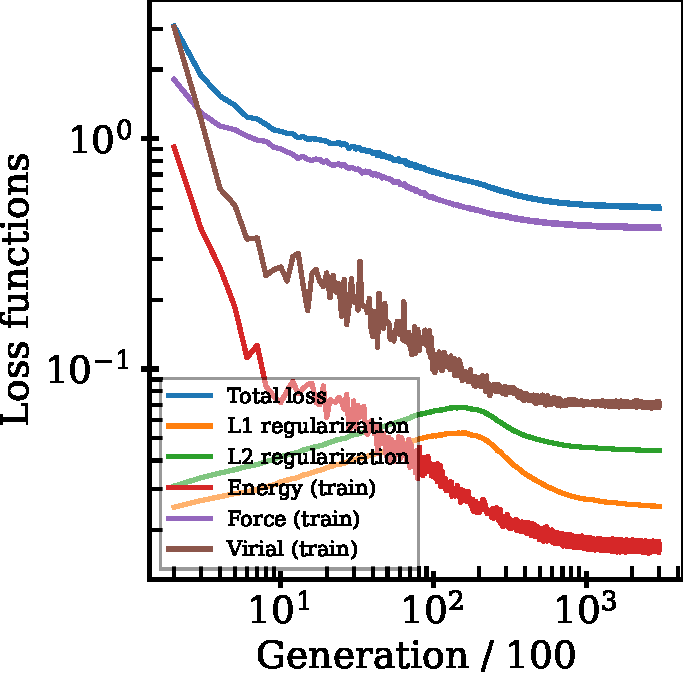
\includegraphics[width=0.6\textwidth]{figures/loss/loss_evolution.pdf}
    \caption{Evolution of training loss as a function of generation, showing total loss and individual contributions from energy, force, virial, and regularization terms.}
    \label{fig:loss_train}
\end{figure}

The accuracy of the trained potential on the training dataset is assessed using parity plots shown in Fig.~\ref{fig:fit_train}. The energy parity plot demonstrates excellent agreement between NEP-predicted and DFT reference cohesive energies. The force parity plot shows that all Cartesian force components are accurately reproduced over a wide force range, which is essential for capturing vibrational and transport properties. The stress parity plot confirms that the model reproduces virial components associated with normal strain (NS$_X$, NS$_Y$) and shear strain (SS$_R$) configurations. The tight clustering of data points around the ideal parity line indicates that the model faithfully reproduces the reference first-principles data included in the training set.

\begin{figure}[htb!]
    \centering
    \subfloat[]{
       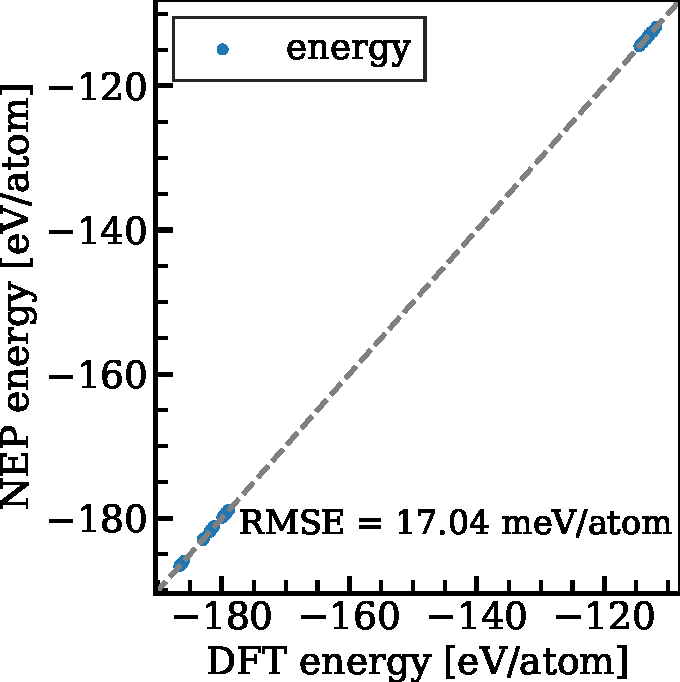
\includegraphics[width=0.45\textwidth]{figures/train/parity_energy.pdf}
    }
    \hfill
    \subfloat[]{
       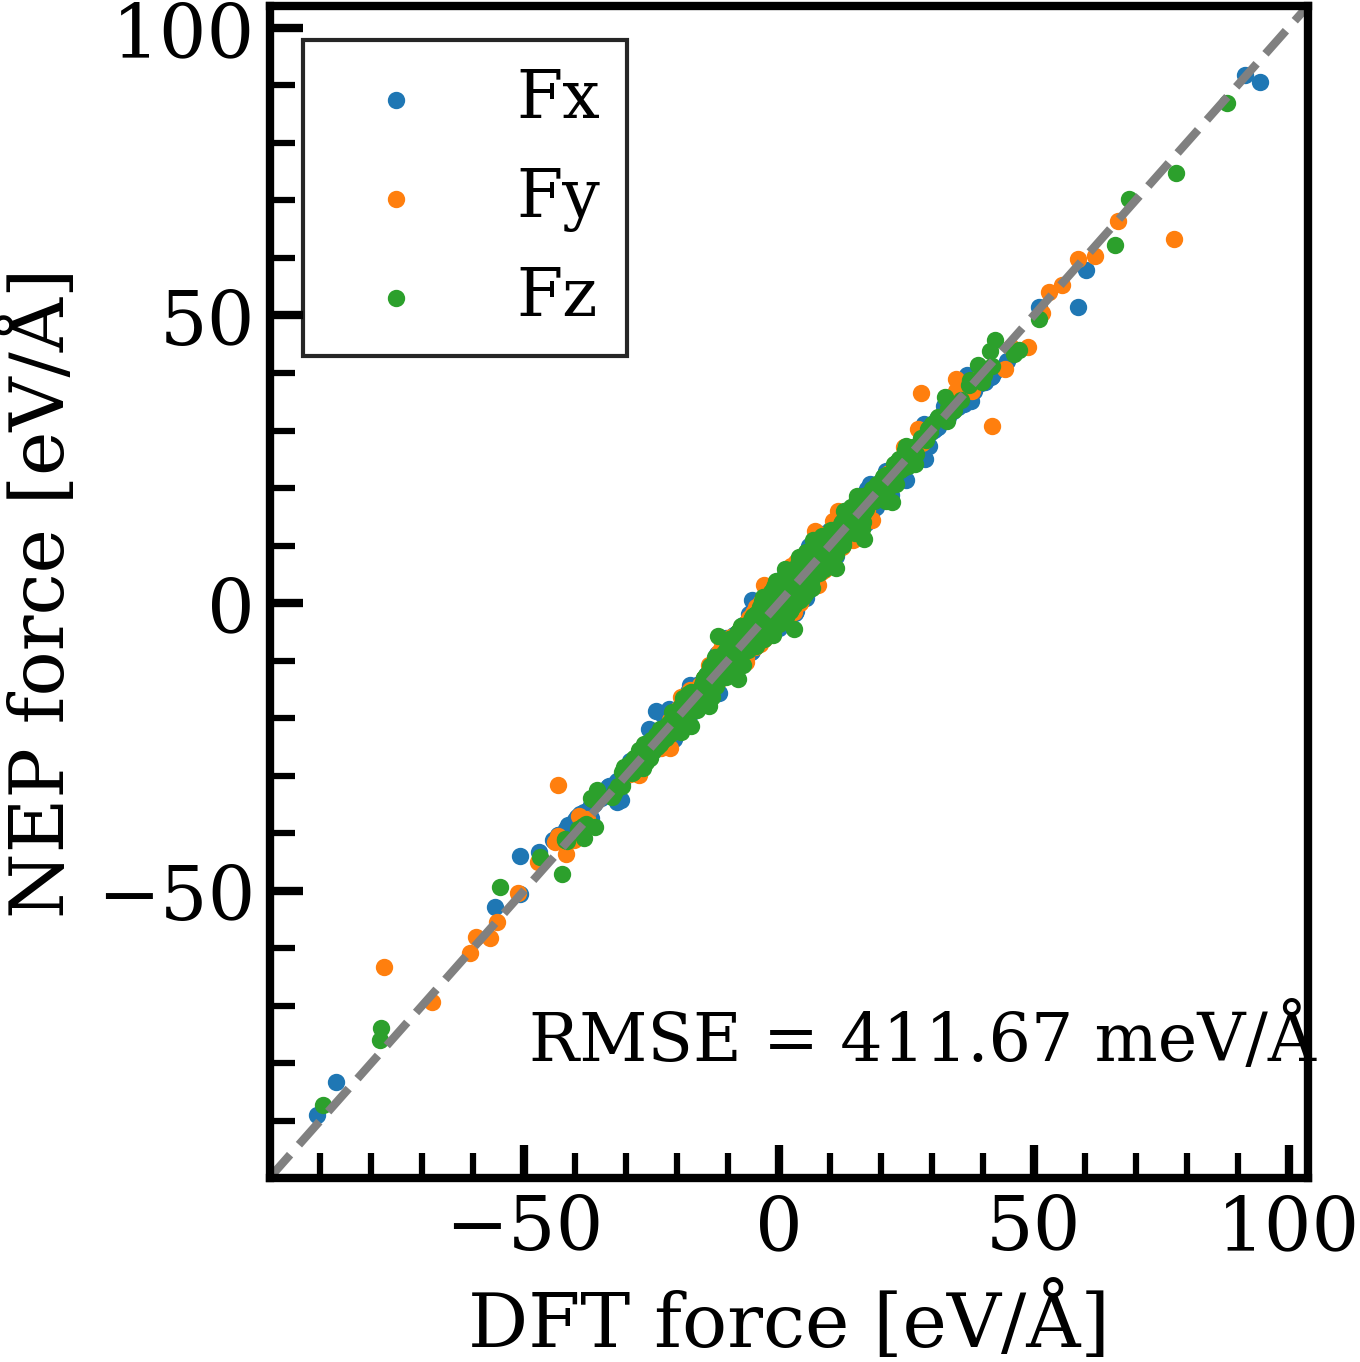
\includegraphics[width=0.45\textwidth]{figures/train/parity_force.png}
    }
    \hfill
    \subfloat[]{
       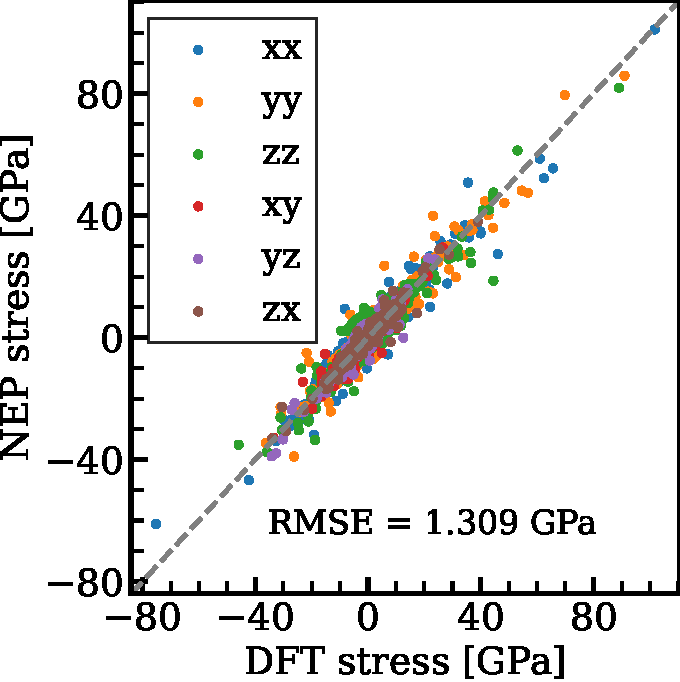
\includegraphics[width=0.45\textwidth]{figures/train/parity_stress.pdf}
    }
    \caption{Parity plots comparing DFT and NEP predictions for the \textbf{training} dataset: 
    (a) cohesive energy $E_{\rm coh}$, 
    (b) atomic force components $F_x, F_y, F_z$, and 
    (c) stress tensor components for supercells belonging to NS$_X$, NS$_Y$, and SS$_R$ deformation modes.}
    \label{fig:fit_train}
\end{figure}

To evaluate the generalization capability of the trained potential, parity plots for an independent test dataset are shown in Fig.~\ref{fig:fit_test}. The close agreement between DFT and NEP predictions for energies, forces, and stresses indicates strong transferability of the potential beyond the configurations included in training. In particular, the force parity plot demonstrates that the learned local environment descriptors remain accurate for unseen atomic configurations, which is critical for reliable molecular dynamics simulations of thermal transport and mechanical deformation. The consistency between training and test errors suggests that the model is not overfitted and is suitable for large-scale atomistic simulations.

\begin{figure}[htb!]
    \centering
    \subfloat[]{
       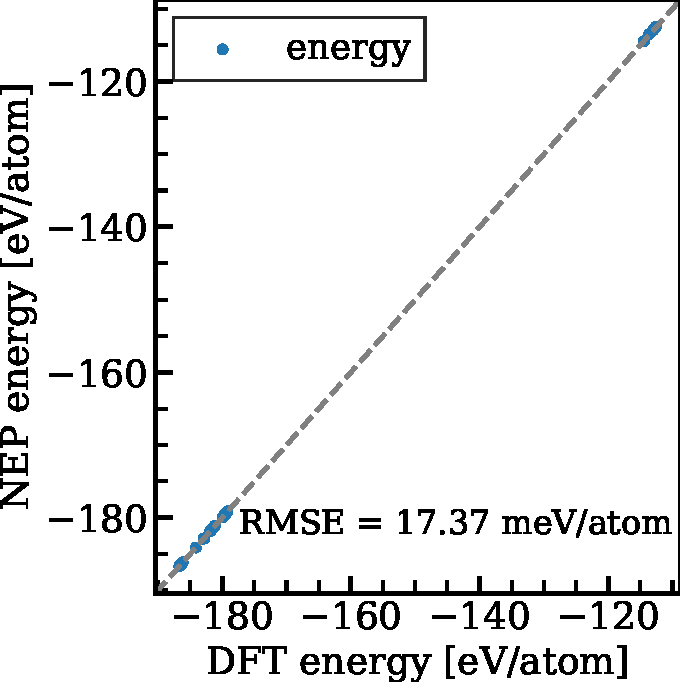
\includegraphics[width=0.45\textwidth]{figures/test/parity_energy_test.pdf}
    }
    \hfill
    \subfloat[]{
       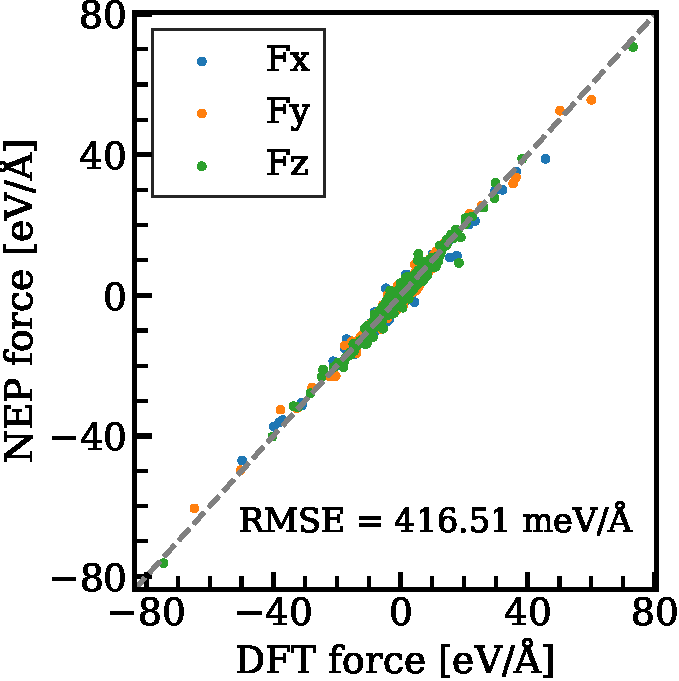
\includegraphics[width=0.45\textwidth]{figures/test/parity_force_test.pdf}
    }
    \hfill
    \subfloat[]{
       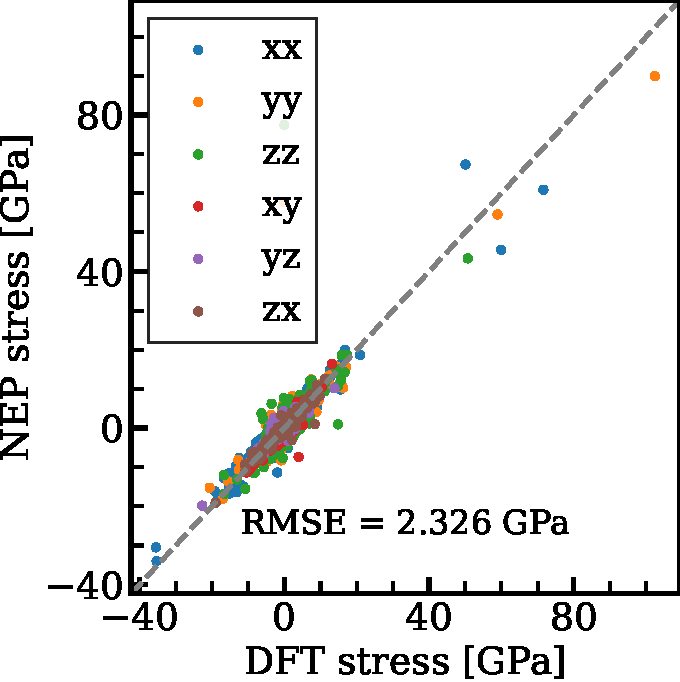
\includegraphics[width=0.45\textwidth]{figures/test/parity_stress_test.pdf}
    }
    \caption{Parity plots comparing DFT and NEP predictions for the \textbf{test} dataset: 
    (a) cohesive energy $E_{\rm coh}$, 
    (b) atomic force components $F_x, F_y, F_z$, and 
    (c) stress tensor components for supercells under NS$_X$, NS$_Y$, and SS$_R$ deformation modes.}
    \label{fig:fit_test}
\end{figure}

\begin{table}[htb!]
\centering
\caption{Comparison of root mean square errors (RMSE) of energy, force, and virial/stress predicted by DeepMD and the present NEP model for training and validation datasets.}
\label{tab:rmse_comparison}
\renewcommand{\arraystretch}{1.2}
\begin{tabular}{lcccc}
\toprule
RMSE Quantity 
& DeepMD (Train) 
& DeepMD (Valid) 
& NEP (Train) 
& NEP (Valid) \\
\midrule
Energy (meV/atom)     
& 1.7   
& 0.455 
& 17.04 
& 17.37 \\

Force (meV/\AA)       
& 34.6  
& 46.7  
& 411.67
& 416.51 \\

Virial / Stress       
& 21.6 meV 
& 2.38 meV 
& 1.309 GPa
& 2.326 GPa\\
\bottomrule
\end{tabular}
\end{table}

While DeepMD provides higher numerical accuracy, especially in force predictions, the NEP model demonstrates stable and comparable errors across training and validation datasets, suggesting robustness and absence of overfitting. Considering its substantially lower computational cost, the NEP potential remains well suited for extensive simulations of lattice dynamics, thermal transport, and mechanical deformation.

The relatively larger cutoff radius and higher angular basis for Mg atoms allow the model to capture longer-range and directional bonding effects across interlayer regions, while the more localized cutoff for Bi reflects its bonding environment. The selected loss weights ensure that force accuracy is prioritized, which is essential for phonon-based thermal conductivity calculations and mechanical property predictions. Overall, the trained NEP model provides an accurate and transferable description of interatomic interactions, enabling reliable molecular dynamics simulations for thermomechanical property evaluation.


\subsection{Molecular Dynamics Simulations in LAMMPS}


\section{Results and Discussion}

\subsection{Validation of the NEP Model}

Compared to DLP, Tersoff, and ExTeP potentials, the present model provides more balanced agreement with reference elastic constants for both in-plane and shear responses, indicating improved transferability for mechanical simulations.


\begin{table}[htb!]
\centering
\caption{Comparison of elastic constants of monolayer of h-BN and bulk c-BN obtained from experiments/DFT and different interatomic potentials.}
\label{tab:elastic_bn}
\renewcommand{\arraystretch}{1.2}
\begin{tabular}{lccccc}
\toprule
 & Exp/DFT & DLP & Tersoff & ExTeP & This Work \\
\midrule
\multicolumn{6}{l}{\textbf{h-BN (Unit: N/m)}} \\
$C_{11}$ & 293.2 & 292.3 & 269.2 & 269.4 & 282.99 \\
$C_{12}$ & 66.1  & 69.5  & 114.7 & 64.8  & 59.32  \\
\midrule
\multicolumn{6}{l}{\textbf{c-BN (Unit: GPa)}} \\
$C_{11}$ & 820 & 691 & 636 & 638 & 613.90 \\
$C_{12}$ & 190 & 192 & 381 & 284 & 165.21 \\
$C_{44}$ & 480 & 400 & 365 & 438 & 463.18 \\
\bottomrule
\end{tabular}
\end{table}

\subsection{RDF}

The radial distribution function (RDF) profiles of the three polymorphs of boron nitride —
amorphous (a-BN), cubic (c-BN), and hexagonal (h-BN) — computed using the NEP potential 
at 0~GPa and 300~K under NVT conditions are shown in Fig.~\ref{fig:rdf_bn}. 
For h-BN, distinct sharp peaks are observed at 1.45, 2.50, 2.89, and 3.82~\AA, 
corresponding respectively to the in-plane B–N covalent bond and successive coordination 
shells within the layered hexagonal lattice. The RDF of c-BN exhibits a well-defined crystalline 
order with pronounced peaks at 1.57, 2.56, 3.01, and 3.63~\AA, characteristic of the tetrahedral 
sp\textsuperscript{3} bonding configuration. In contrast, a-BN displays broadened and less intense 
peaks located near 1.46, 2.53, and 3.81~\AA, indicating only short-range order and the absence 
of long-range periodicity typical of the amorphous phase. These RDF results clearly demonstrate 
that the NEP potential accurately captures the local atomic correlations of all three BN 
polymorphs, reproducing both the sharp first-neighbor peak positions and the expected 
structural disorder in a-BN. The excellent agreement with previously reported experimental 
and DFT-based RDF features confirms the robustness of the NEP potential in modeling 
structural properties across both crystalline and amorphous phases of boron nitride.


\begin{figure}[htb!]
    \centering
    \subfloat[]{
       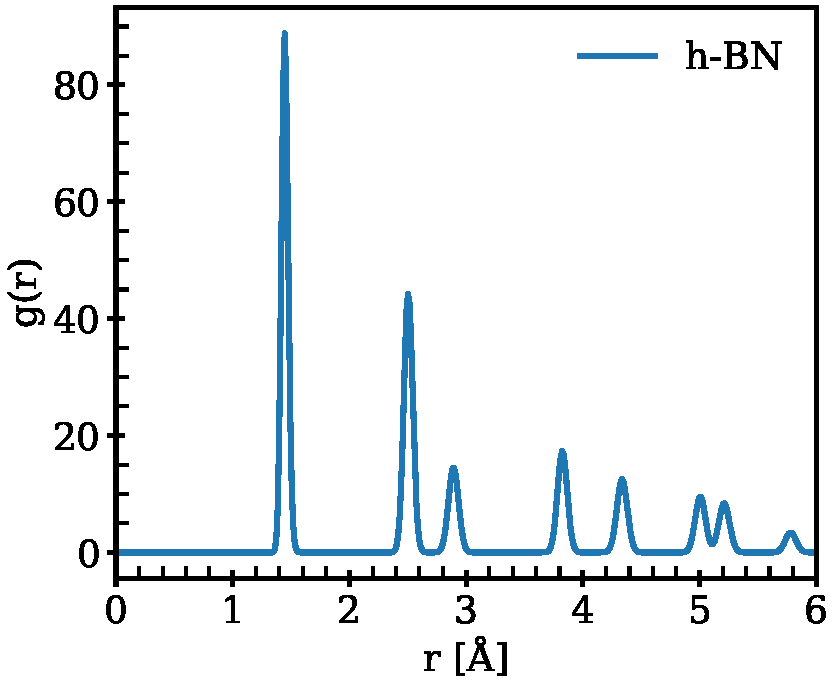
\includegraphics[width=0.45\textwidth]{figures/rdf/rdf_h-BN.pdf}
    }
    \hfill
    \subfloat[]{
       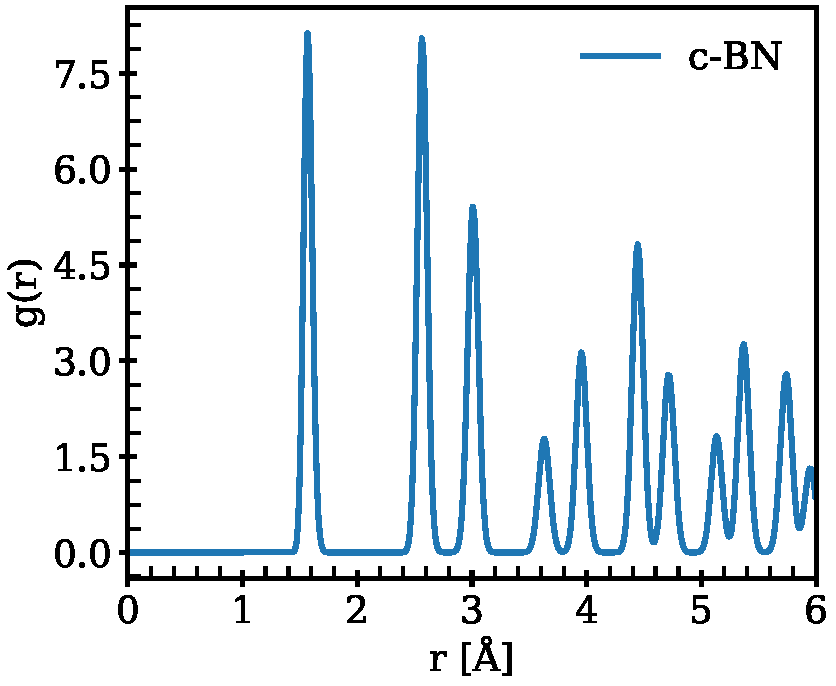
\includegraphics[width=0.45\textwidth]{figures/rdf/rdf_c-BN.pdf}
    }
    \hfill
    \subfloat[]{
       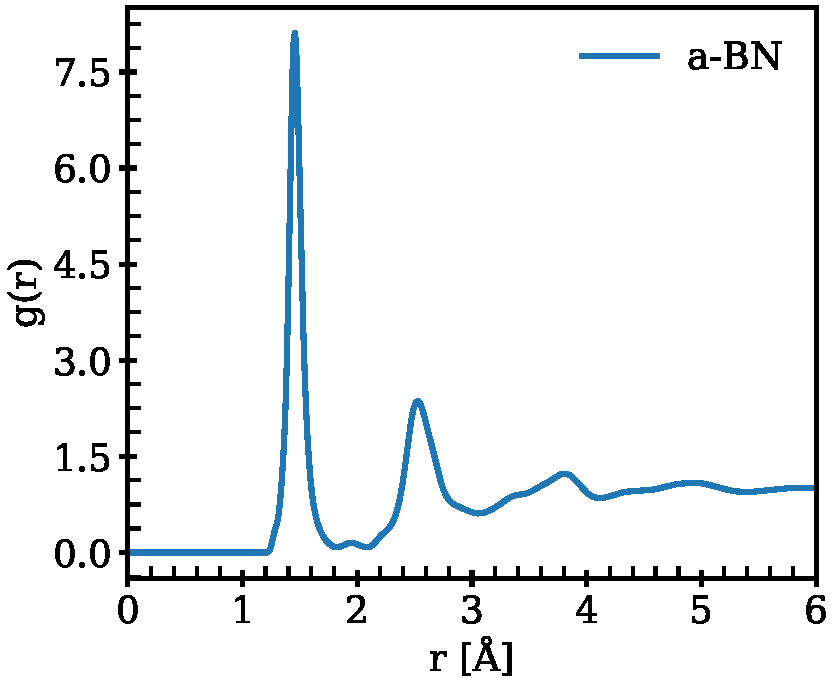
\includegraphics[width=0.45\textwidth]{figures/rdf/rdf_a-BN.pdf}
    }
    \caption{
    Radial distribution function (RDF) profiles of (a) monolayer h-BN (mp-7991), 
    (b) c-BN (mp-1639), and (c) a-BN (mp-1244991) obtained using the NEP potential 
    at 0~GPa and 300~K under NVT ensemble. 
    The RDFs exhibit the characteristic short-range order of each polymorph, 
    demonstrating the NEP potential’s ability to accurately reproduce structural correlations.
    }
    \label{fig:rdf_bn}
\end{figure}


\subsection{Elastic Properties of Amorphous BN}


\begin{table}[h!]
\centering
\caption{Variation of elastic modulus, goodness of fit, and ultimate strength with density.}
\label{tab:mechanical_density}
\begin{tabular}{ccccc}
\toprule
\textbf{Density} &
\textbf{Young's Modulus (GPa)} &
\textbf{$R^2$} &
\textbf{$\sigma_{\max}$ (GPa)} &
\textbf{$\varepsilon$ at $\sigma_{\max}$} \\
\midrule
0.80 & 5.53  & 0.99008 & 3.91  & 0.638 \\
1.00 & 25.35 & 0.98707 & 4.00  & 0.402 \\
1.30 & 51.71 & 0.99770 & 8.51  & 0.330 \\
1.60 & 74.67 & 0.99323 & 7.71  & 0.434 \\
2.00 & 90.62 & 0.98338 & 12.54 & 0.120 \\
2.30 & 104.63 & 0.99714 & 10.75 & 0.126 \\
\bottomrule
\end{tabular}
\end{table}




\begin{figure}[htb!]
    \centering
    % --- First row ---
    \subfloat[density 0.80]{
        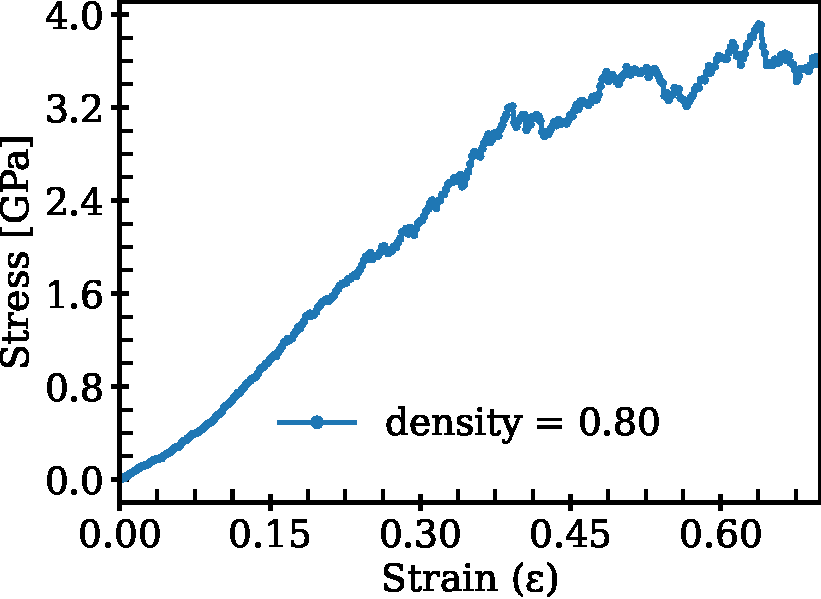
\includegraphics[width=0.45\textwidth]{figures/tensile/Pzz_vs_Strain_density_0.80.pdf}
    }
    \hfill
    \subfloat[density 1.00]{
        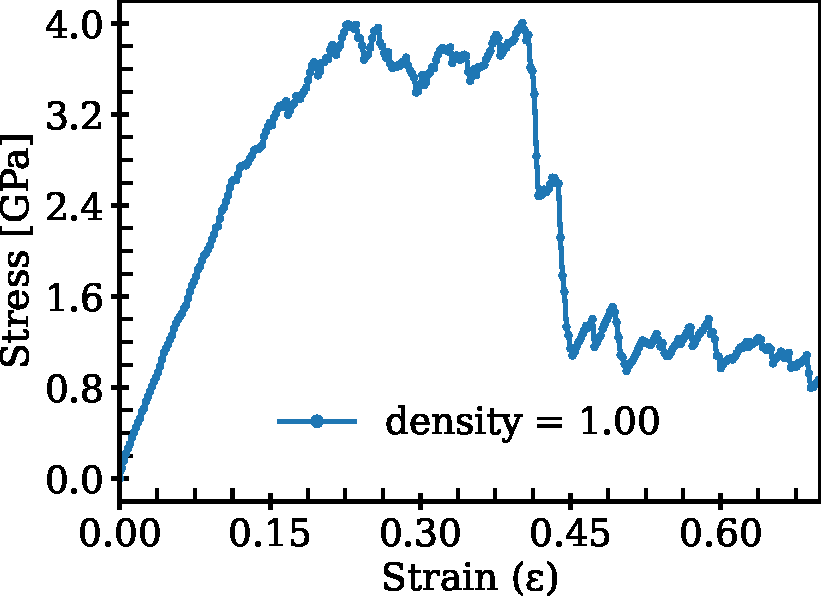
\includegraphics[width=0.45\textwidth]{figures/tensile/Pzz_vs_Strain_density_1.00.pdf}
    }
    \\[1em] % space between rows

    % --- Second row ---
    \subfloat[density 1.30]{
        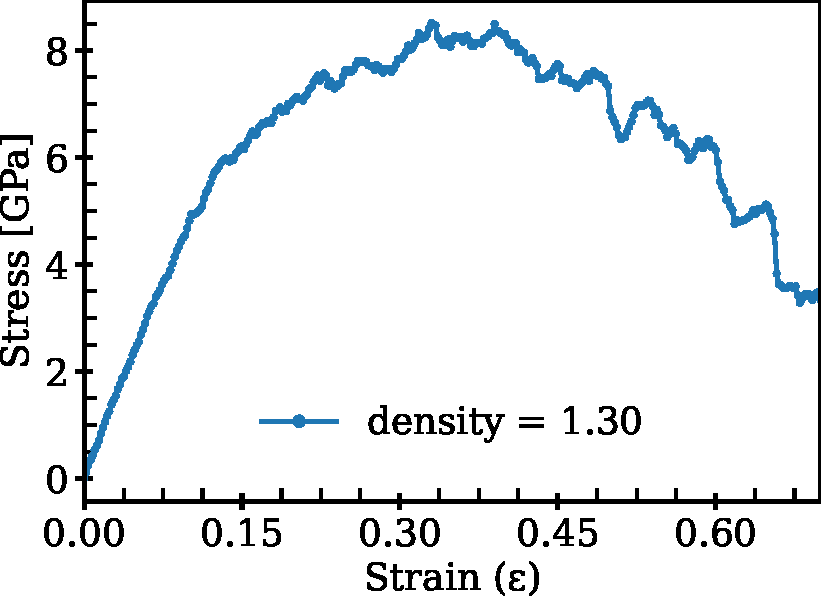
\includegraphics[width=0.45\textwidth]{figures/tensile/Pzz_vs_Strain_density_1.30.pdf}
    }
    \hfill
    \subfloat[density 1.60]{
        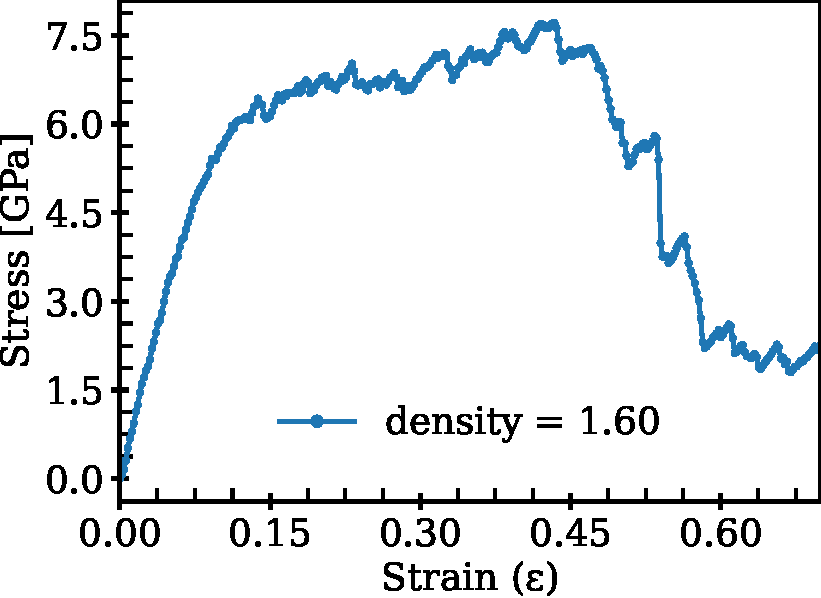
\includegraphics[width=0.45\textwidth]{figures/tensile/Pzz_vs_Strain_density_1.60.pdf}
    }
    \\[1em]

    % --- Third row ---
    \subfloat[density 2.00]{
        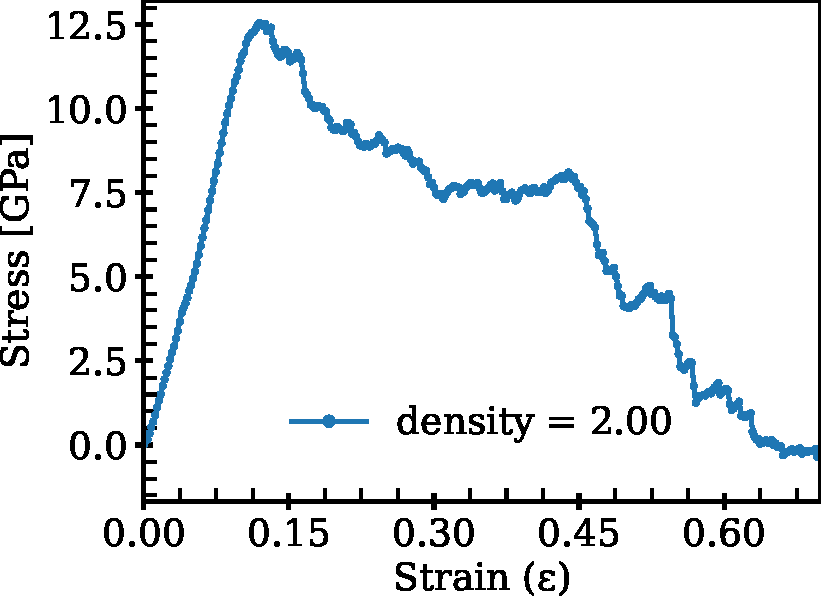
\includegraphics[width=0.45\textwidth]{figures/tensile/Pzz_vs_Strain_density_2.00.pdf}
    }
    \hfill
    \subfloat[density 2.30]{
        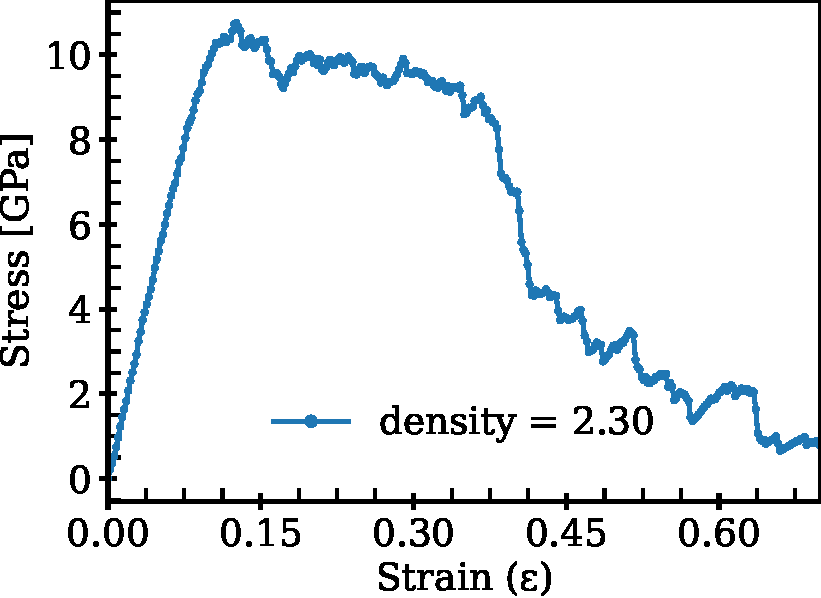
\includegraphics[width=0.45\textwidth]{figures/tensile/Pzz_vs_Strain_density_2.30.pdf}
    }

    \caption{
        Stress–strain curves for h-BN nanoporous structures with different initial densities:
        (a)~0.80, (b)~1.00, (c)~1.30, (d)~1.60, (e)~2.00, and (f)~2.30~g/cm$^3$. 
        Each curve shows the tensile response computed from MD simulations.
    }
    \label{fig:tensile_density}
\end{figure}

\subsection{Stress--Strain Response Under Uniaxial Loading}
% Tensile curves at different densities

\subsection{Atomic-Scale Deformation and Fracture Mechanisms}
% Local shear strain, crack initiation

\subsection{Comparison with DeepMD-Based Results}

The computational efficiency of the proposed NEP model was evaluated using large-scale molecular dynamics simulations within the LAMMPS framework. For a system containing 3,072 atoms, the NEP-based simulation completed within 3.05 hours, whereas a neural network potential (NNP) required approximately 24 hours under comparable computational resources, corresponding to an almost eight-fold speedup. Furthermore, for a larger system consisting of approximately 12,500 atoms, the NEP model completed the simulation within 5.8 hours, demonstrating near-linear scaling with system size. These results highlight the superior computational efficiency and scalability of the NEP framework for large-scale atomistic simulations.

\begin{table}[h!]
\centering
\caption{Comparison of computational performance of NNP and NEP models.}
\label{tab:performance}
\begin{tabular}{lccccc}
\hline
Potential & Atoms & Nodes & Cores & Time (hrs) & Speedup \\
\hline
NNP & 3072 & 20 & 960 & 24.0 & 1.0 \\
NEP & 3072 & 20 & 960 & 3.05 & 7.9 \\
NEP & 12500 & 20 & 960 & 5.8 & -- \\
\hline
\end{tabular}
\end{table}


\section{Conclusions}



%%%%%%%%%%%%%%%%%%%%%%%%%%%%%%%%%%%%%%%%%%%%%%%%%%%%%%%%%
\section*{Acknowledgment}
The authors appreciate the financial support and computing resources of IIT Bombay. Views expressed in this paper are those of the authors and neither of their affiliated institutions nor of the funding agencies.

\section*{Declaration of Generative AI and AI-assisted technologies in the writing process}
During the manuscript preparation, the authors used ChatGPT (OpenAI) to assist in English language editing and the overall structure of the text. The scientific ideas, data analysis, and conclusions presented herein are solely those of the authors, who assume full responsibility for the content.

\bibliographystyle{elsarticle-num} 
\bibliography{references.bib}

\end{document}
